\subsection{Módulo de Recomendación Nutricional Adaptativo}
\label{sec:modulo_nutricion}

El módulo de recomendación nutricional tiene como propósito principal mitigar los índices de anemia ferropénica infantil y desnutrición crónica en zonas vulnerables. Para ello, implementa un motor de toma de decisiones local y offline basado en una base de datos relacional SQLite gestionada por el servicio \texttt{dbService.ts}. El flujo metodológico y los componentes de este módulo se estructuran en tres dimensiones fundamentales:

\subsubsection{Catálogo Nutricional y Mapeo por Ecorregiones}
La base de datos local se inicializa con un catálogo sembrado de 15 alimentos andinos y amazónicos representativos del Perú (obtenidos de las Tablas Peruanas de Composición de Alimentos (TPCA) del INS~\cite{INS2023}), clasificados en grupos biológicos (vísceras, carnes, legumbres, pseudocerales, frutas, semillas y pescados). Cada registro alimentario (\texttt{Alimento}) contiene 24 campos que incluyen macronutrientes, micronutrientes esenciales (hierro hemínico, hierro no hemínico, vitamina C, zinc y calcio), costo estimado por kilogramo, estacionalidad, tiempo de conservación y presencia de alérgenos comunes.

Para garantizar la disponibilidad física y pertinencia cultural de las recomendaciones, el sistema integra la clasificación de las 11 Ecorregiones del Perú propuesta por Antonio Brack Egg~\cite{brack1986ecorregiones}. Mediante la tabla relacional de asociación \texttt{alimento\_ecorregion}, el motor de recomendación filtra los alimentos según la ubicación geográfica del paciente:
\begin{itemize}
    \item \textbf{Mar Frío de la Corriente Peruana}: Priorización de la Anchoveta por su alta concentración de proteínas, hierro y Omega-3 (DHA/EPA).
    \item \textbf{Puna y Altos Andes}: Selección de pseudocereales y leguminosas adaptados a altitudes superiores a los 3800 m.s.n.m., como la Quinua, Kiwicha, Cañihua y el Tarwi (chocho), ricos en aminoácidos esenciales y calcio.
    \item \textbf{Selva Alta y Selva Baja}: Inclusión de frutas nativas como el Camu Camu (fuente crítica de vitamina C con 2780 mg por 100g para potenciar la absorción de hierro no hemínico) y pescados de río como el Paiche.
    \item \textbf{Serranía Esteparia y Desierto del Pacífico}: Acceso a carnes magras como el Cuy, vísceras y legumbres locales (lentejas, habas).
\end{itemize}

\subsubsection{Motor de Sustitución Inteligente de Bajo Costo}
A fin de optimizar el presupuesto familiar de los hogares rurales, el módulo incorpora un algoritmo de sustitución inteligente (\texttt{sustituciones}) regulado por coeficientes nutricionales y económicos. El sistema calcula la equivalencia en gramos ($E_g$) y el ahorro porcentual esperado ($A_{\%}$) al reemplazar un alimento costoso o ausente por una alternativa local. El algoritmo opera bajo el siguiente criterio de optimización:
\begin{equation}
    E_g = C_o \cdot \frac{Fe_{\text{original}}}{Fe_{\text{sustituto}}}
\end{equation}
donde $C_o$ es la porción original de referencia en gramos, y $Fe$ representa el contenido de hierro disponible por cada gramo de alimento. Por ejemplo, el motor sugiere sustituir el lomo de res (alimento de costo elevado y con solo 3.0 mg de hierro por 100g) por la sangrecita de pollo cocida (víscera de bajo costo que aporta 29.5 mg de hierro hemínico por 100g). Esta sustitución específica reduce el costo del plato en un 85\% e incrementa la concentración de hierro biodisponible en casi 10 veces, facilitando la adherencia clínica sin comprometer la economía del hogar.

\subsubsection{Lógica de Recomendación Clínica y Recetario Dinámico}
Una vez obtenido el nivel de anemia en el diagnóstico (estimado en la conjuntiva ocular), la interfaz (\texttt{NutritionScreen.tsx}) recupera de manera reactiva el catálogo local y ejecuta el árbol de decisión clínica:
\begin{enumerate}
    \item \textbf{Estado Anémico Severo o Moderado}: El motor realiza un filtro estricto sobre alimentos cuyo campo \texttt{estado\_nutricional\_objetivo} incluya el tag \texttt{"Anemia"} o que posean un nivel de hierro total (hemínico + no hemínico) mayor a 2.0 mg por 100g. Simultáneamente, el sistema sugiere guías de suplementación en gotas o jarabe (ej. Hierro Terapéutico a razón de 2 mg/kg/día para casos moderados, y derivación de urgencia médica para casos severos).
    \item \textbf{Estado Normal / Preventivo}: El filtrado se orienta a alimentos orientados a combatir la desnutrición crónica y promover el crecimiento cognitivo (pseudocereales, semillas y frutas ricas en zinc y calcio), sugiriendo dosis profilácticas preventivas de sulfato ferroso.
\end{enumerate}

El sistema asocia el diagnóstico a un recetario embebido en memoria (\texttt{RECIPES\_DB}), proponiendo platos típicos formulados para la edad del paciente (ej. Papilla de Hígado de Pollo y Zapallo para lactantes con diagnóstico severo; Guisito de Lentejas con Bofe o Crema de Habas con Sangrecita para estados moderados; y Mazamorra de Quinua con Durazno para prevención). 

Finalmente, el usuario puede seleccionar libremente alimentos del catálogo para estructurar una dieta personalizada. Al guardar la recomendación o la dieta configurada, el sistema serializa el objeto en formato JSON y lo registra en la tabla local \texttt{historial\_dietas} de SQLite, quedando listo para ser transmitido al servidor central durante la siguiente sincronización mesh.

La interfaz de usuario del módulo de nutrición y recetario se ilustra en la Figura~\ref{fig:mod_nutricion}.

\begin{figure}[H]
\centering
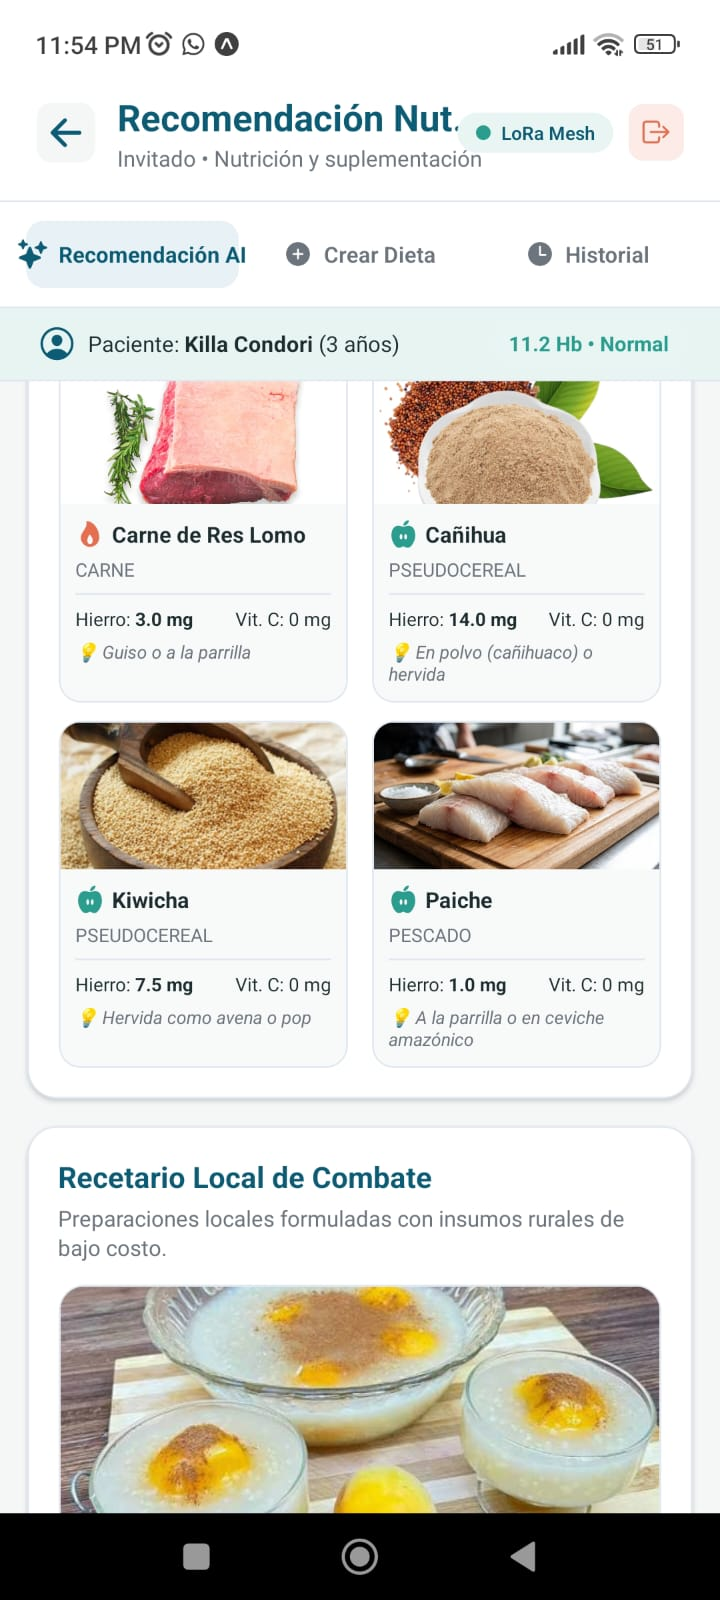
\includegraphics[width=0.28\textwidth]{images/Nutricion.jpeg}
\caption{Interfaz del Módulo de Recomendación Nutricional y Recetario Local}
\label{fig:mod_nutricion}
\end{figure}

